%!TEX root = ../report.tex
\documentclass[../report.tex]{subfiles}
\begin{document}
    \chapter{Implementation}\label{ch_implementation}
    This chapter describes gives implementation details of the experiments conducted during this thesis work. In the beginning training details of the GestaltMatcher model are provided. Subsequently, we describe the procedure to integrate explanation methods with the model. Furthermore, implementation details of the experiments proposed in the previous chapter are discussed. Finally, the evaluation questionnaire is presented.
	\section{GestaltMatcher Model Training}
%	\begin{figure}[ht]
%		\hspace*{-0.5cm}      
%		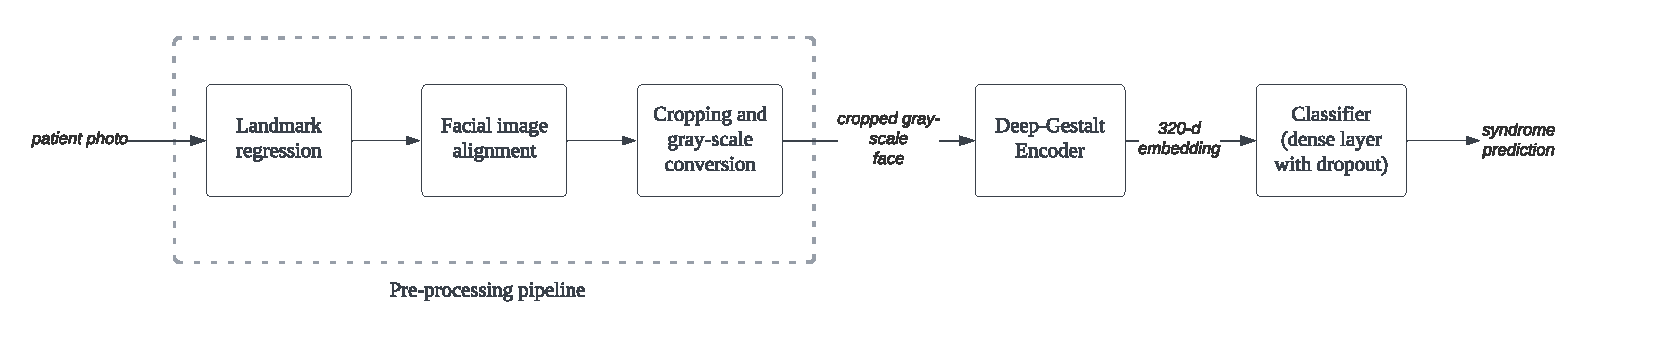
\includegraphics[scale=0.62]{chapter4/gestalt_classifier_pipeline.pdf}
%		\caption{Illustration of the pipleline to process a patient photo using GestaltMatcher}
%		\label{fig_cl_pipeline}
%	\end{figure}
	The architecture and working of GestaltMatcher was explained in Chapter \ref{chap_background}. This work uses the classifier variant of GestaltMatcher for its experiments (refer Figure \ref{fig_arch_gest_matcher} for architectural details). The neural network is first trained on facial images from the CASIA-WebFace \cite{yi2014learning} dataset. Subsequently, it is trained on 139 frequent-syndrome classes listed by the authors of GestaltMatcher. The training details are presented in Table \ref{tab_learning_details}.
	
	\begin{table}[H]
		\centering
		\begin{tabular}{|l|l|}
			\hline
			\textbf{Hyperparameter} & \textbf{Value}                                                         \\ \hline
			Loss function           & \begin{tabular}[c]{@{}l@{}}weighted \\ cross entropy loss\end{tabular} \\ \hline
			Input image size        & 100 x 100                                                              \\ \hline
			Batch size              & 280                                                                    \\ \hline
			Epochs                  & 200                                                                    \\ \hline
			Learning rate           & 0.05                                                                   \\ \hline
			Momentum                & 0.9                                                                    \\ \hline
		\end{tabular}
	\caption{GestaltMatcher classifier training details}
	\label{tab_learning_details}
	\end{table}

    \section{Explanation Methods - GestaltMatcher Integration}
     \begin{figure}[H]
    	\hspace*{0.5cm}      
    	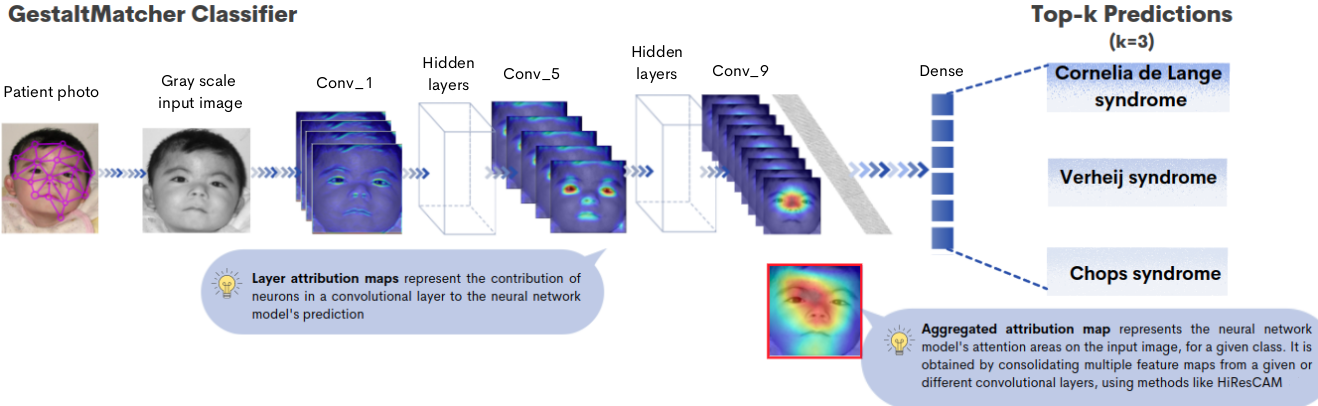
\includegraphics[scale=0.45]{chapter5/xai_gestalt_matcher_intergration.png}
    	\caption{An illustration of attribution map computation from the GestaltMatcher model}
    	\label{fig_gm_pipeline}
    \end{figure}
	The Class Activation Mapping (CAM) methods used for this work typically generate class-specific attribution maps, by evaluating contributions of neurons in a given convolutional layer to the model output. Therefore, the choice of target convolutional layer plays a vital role. Selvaraju \etal \cite{selvaraju2017grad} recommend to use the last convolutional layers, as they contain more high-level semantic and spatial information, when compared to earlier layers, which have smaller receptive fields. The same is reinforced by Muhammad \etal \cite{muhammad2020eigen}. We validated this recommendation by computing and comparing attribution maps generated from all ten convolutional layers, using both GradCAM and HiResCAM techniques. FullGrad was excluded from this analysis, as the method is layer-agnostic in nature.

	Based on the recommendation and our observations, we chose layer 14 (refer conv\_9 in Figure \ref{fig_layer_visual}), the last convolutional layer to compute attribution maps.\\
	\subsubsection{CustomGradCAM}
	Apart from the last convolution layer, we also observed that applying GradCAM to layers 10.a and 11.a produced visualizations in which certain key features of human face are highlighted (refer conv\_6 and conv\_7 in Figure \ref{fig_layer_visual}). Therefore, in order to include the layers in our scope, we averaged their attribution maps along with the ones produced by layer 14. The resulting map is presented under the name of \enquote{CustomGradCAM}. We used the Application Programming Interfaces (APIs) offered by PyTorch \cite{paszke2019pytorch}, Captum \cite{kokhlikyan2020captum} and an open-source library \cite{jacobgilpytorchcam} to integrate the explanation methods to the GestaltMatcher classifier model.
	\begin{figure}[H]
		\hspace*{1.0cm}      
		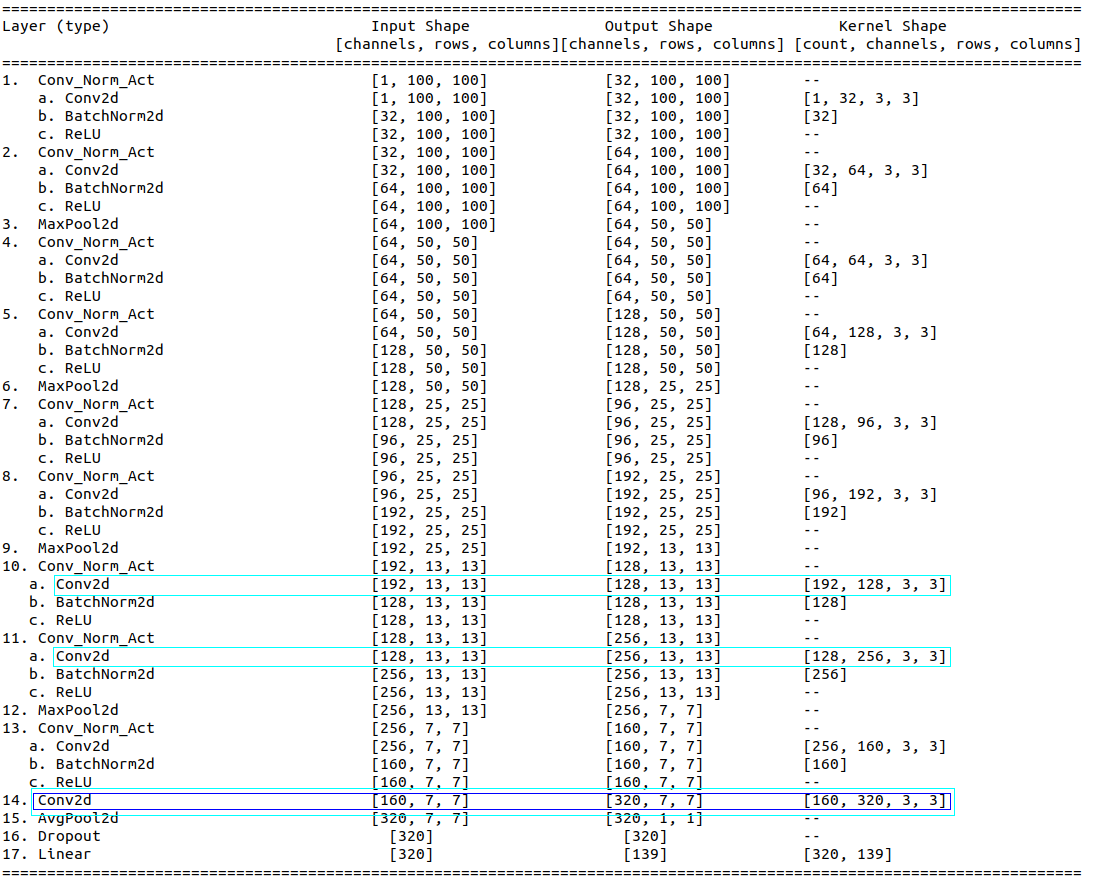
\includegraphics[scale=0.4]{chapter5/gestalt_matcher_arch.png}
		\caption{Architecture of GestaltMatcher classifier. The convolution layer 14 used to generate attribution maps using GradCAM and HiResCAM methods is highlighted using a blue box. Layers (10.a, 11.a and 14) that are used by the CustomGradCAM method are highlighted using cyan boxes. }
		\label{fig_arch_gest_matcher}
	\end{figure}
	\begin{sidewaysfigure}
	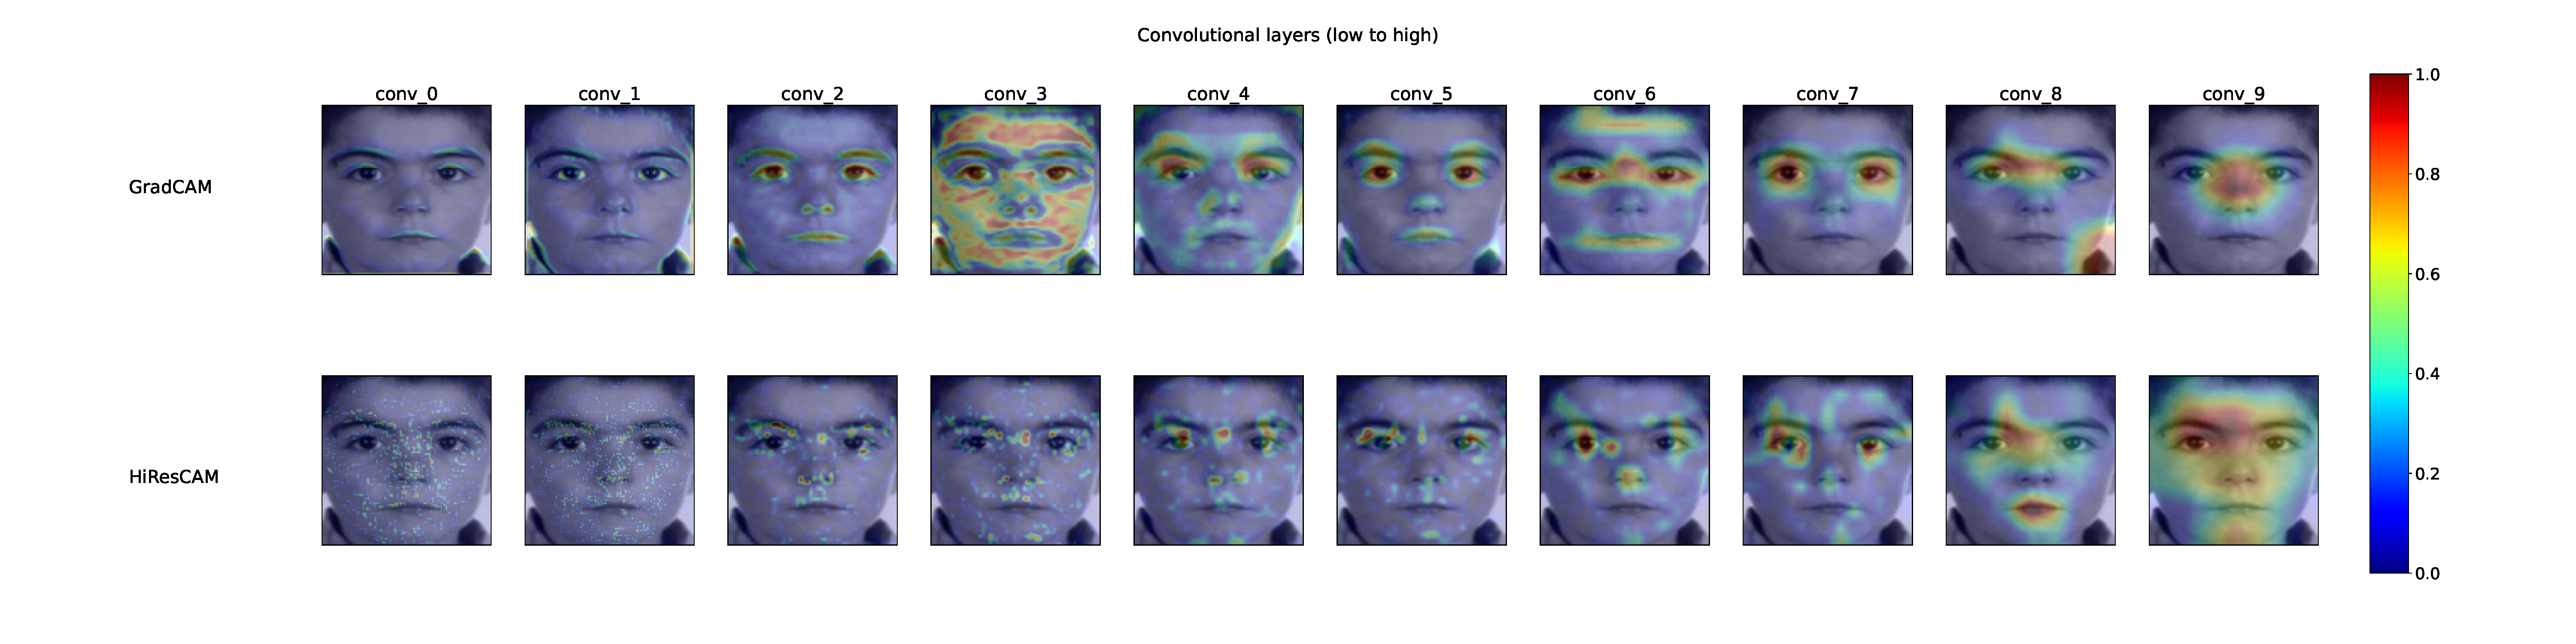
\includegraphics[scale=0.22, trim = 1cm 2.50cm 1cm 2.50cm, clip]{chapter5/layer_attribution1_synd1.pdf}
	
	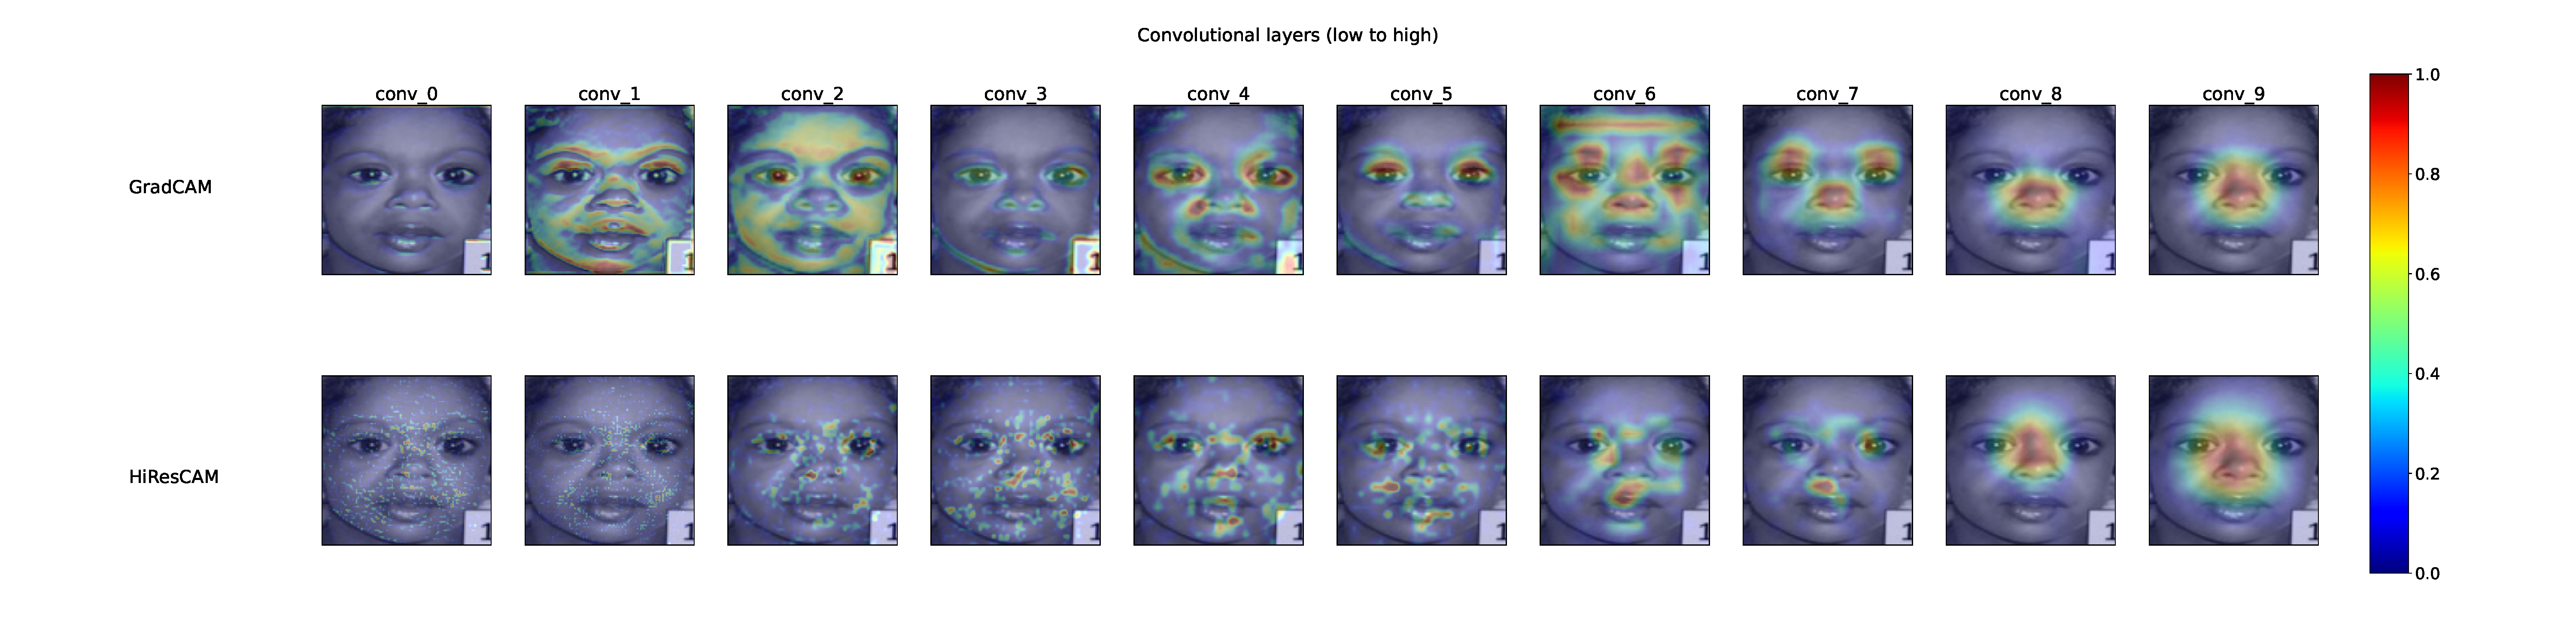
\includegraphics[scale=0.22, trim = 1cm 2.50cm 1cm 2.50cm, clip]{chapter5/layer_attribution3_synd1.pdf}
	\label{fig_gm_pipeline}	      
	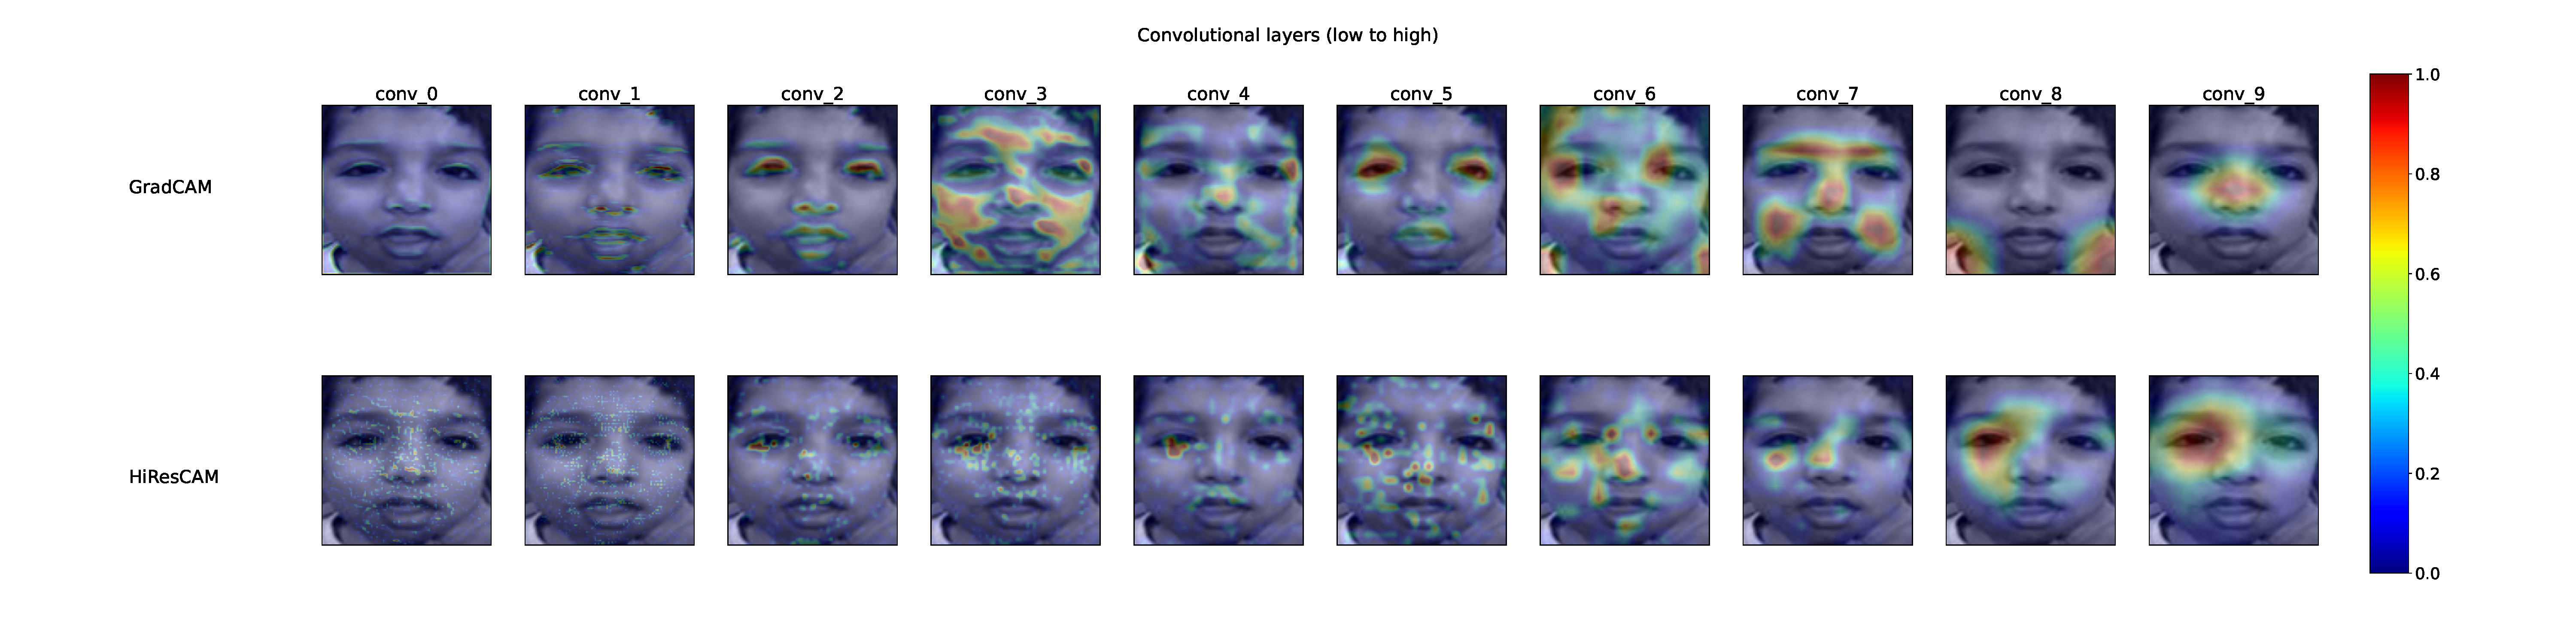
\includegraphics[scale=0.22, trim = 1cm 2.50cm 1cm 2.50cm, clip]{chapter5/layer_attribution_synd2.pdf}
	\caption{Layer-wise visualization of attribution maps generated by GradCAM and HiResCAM methods.}
	\label{fig_layer_visual}
\end{sidewaysfigure}
	\subsection{Visualization Details}
	 Captum's visualizer tool was used to generate color coded attribution maps. We post-processed attribution maps to remove noise and visual artifacts. This section provides details on visualization parameters and the post-processing procedure.
	\subsubsection{Interpolation}
	The attribution maps generated by layer-specific methods such as GradCAM and HiResCAM are shaped identical to the feature maps outputted by the target layers. For example, layer 14 of the gestaltmatcher model spits out 320 7x7 (height x width) feature maps, and any attribution map generated from the layer is of dimensions 7x7 (height x width). The bilinear interpolation technique \cite{bovik2009essential} was used to rescale attribution maps to the input image size of 100x100 (height x width), so that the map could be overlaid on the input image.
	\subsubsection{Attribution Sign and Representation}
	We considered only positive attribution values for visualization and used the \enquote{jet} colormap scheme offered by Captum's \cite{kokhlikyan2020captum} visualization tool.
	\subsubsection{Smoothing Attribution Maps}
	Test Time Augmentation (TTA) is a commonly used technique to boost the performance of image classification models \cite{simonyan2014very}. During the inference process for a given input image, instead of passing the actual sample, its augmented counterparts are fed to obtain predictions from the model. Thus obtained predictions are averaged to obtain the final output. Augmented copies are obtained by applying transformations such as rotations and flips to the original input image.\\
	In our work, we used TTA to enhance the quality of generated attribution maps. Augmented copies of every test input image were obtained by individually applying horizontal flipping and multiplications (with factors of 0.9, 1 and 1.1) operations. Attribution maps were generated for each augmented copy, and finally averaged to obtain the smoothened map. Attribution maps produced from HiResCAM were exempted from TTA based on the guidelines provided by Jacob Gildendblat \cite{jacobgilpytorchcam}.
	
    \section{Experiments}
    Implementation details of the conducted set of experiments are presented in this section.
    \subsection{A. Patient-wise Attribution Map Generation}
    Patient-wise attribution maps are generated by applying the chosen set of methods to individual patient images. The attributions are computed with respect to the logit scores of the samples' ground truth classes. This is because the attribution \enquote{methods work only when the classification result is correct} \cite{muhammad2020eigen}. However, an experiment was also conducted to observe the differences between explanations of misclassified samples, obtained by computing attributions with respect to their ground truth and predicted labels. Its results are discussed in the next chapter.
    \begin{figure}[H]
    	\hspace*{0cm}      
    	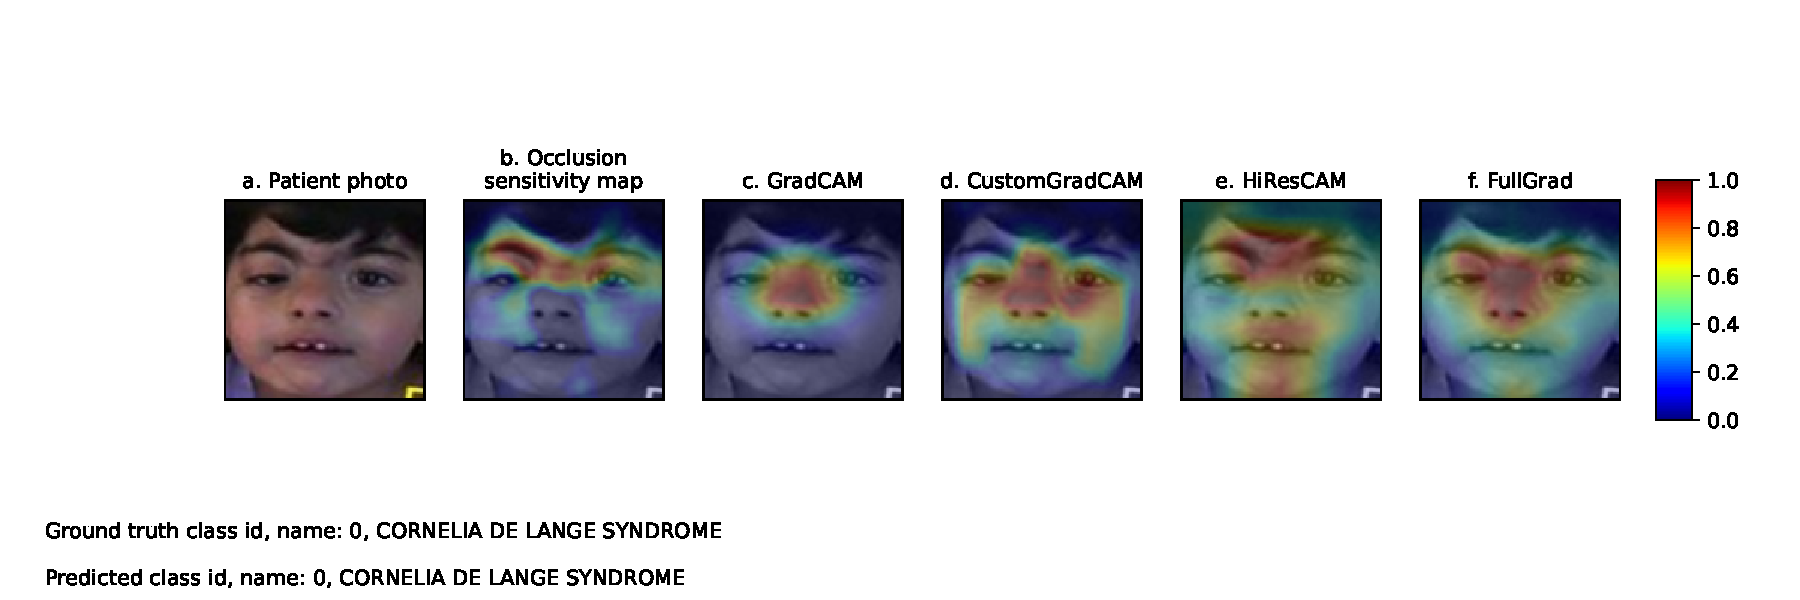
\includegraphics[scale=0.55,trim = 1cm 2.50cm 1cm 2.50cm, clip]{chapter5/example_attribution.pdf}
    	\caption{An example for patient-wise attribution maps}
    	\label{fig_gm_pipeline}
    \end{figure}
    \subsection{B. Composite Face Generation}
    Composite faces are generated with an intent to synthesize a characteristic face for each genetic syndrome class under our scope. Concisely put, they are obtained from aligning and averaging facial images of each category separately. This section provides a detailed description of the process involved.
       \begin{figure}[H]
    	\hspace*{-0.5cm}      
    	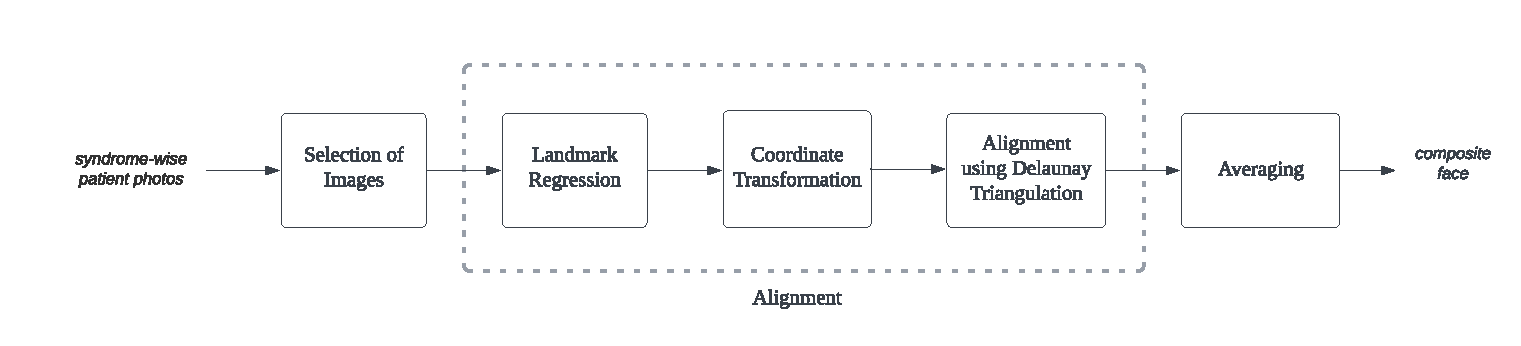
\includegraphics[scale=0.66]{chapter5/composite_face_pipeline.pdf}
    	\caption{Block diagram representing composite face generation process}
    	\label{fig_gm_pipeline}
    \end{figure}
    
    \subsubsection{a. Selection of Images}
    The first step involved in generating composite faces is to select the right consituent images. A considerable number of images in GestaltMatcherDataBase (GMDB) are characterized by poor visual quality and/or presence of artifacts. A few such as the ones shown in Figure \ref{fig_gmdb_poorq} also contain objects like nasal catheter tubes, spectacles, and black strips which were introduced to conceal patient identities. Therefore, we hand picked images from each of 139 syndrome classes to remove the unsuitable candidates for generating composite faces.
    
       \begin{figure}[H]
    	   	\centering
    	   	\begin{subfigure}[b]{0.17\textwidth}
    		   		\centering
    		   		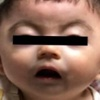
\includegraphics[width=\textwidth]{chapter5/poor_1.jpg}
    		   	\end{subfigure}
    	   	\begin{subfigure}[b]{0.17\textwidth}
    		   		\centering
    		   		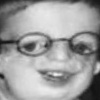
\includegraphics[width=\textwidth]{chapter5/poor_2.jpg}
    		   	\end{subfigure}
    	   		\begin{subfigure}[b]{0.17\textwidth}
    	   		\centering
    	   		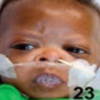
\includegraphics[width=\textwidth]{chapter5/poor_3.jpg}
    	   	\end{subfigure}
       		\begin{subfigure}[b]{0.17\textwidth}
       			\centering
       			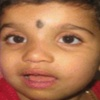
\includegraphics[width=\textwidth]{chapter5/poor_4.jpg}
       		\end{subfigure}
       			\begin{subfigure}[b]{0.17\textwidth}
       			\centering
       			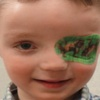
\includegraphics[width=\textwidth]{chapter5/poor_5.jpg}
       		\end{subfigure}
    	   	\caption{Examples of images rejected for composite face generation}
    	   	\label{fig_gmdb_poorq}
    	   \end{figure}
    \subsubsection{b. Facial Landmark Regression}
    Landmark points act as anchors to align the constituent images of composite faces. 68 landmark points are calculated for each input facial image using the dlib \footnote{dlib library - \url{http://dlib.net/}.}library's face detector functionality. Internally, dlib uses a CNN based max-margin object detector to perform the task.
        \begin{figure}[H]
        \centering
    	\hspace*{0cm}      
    	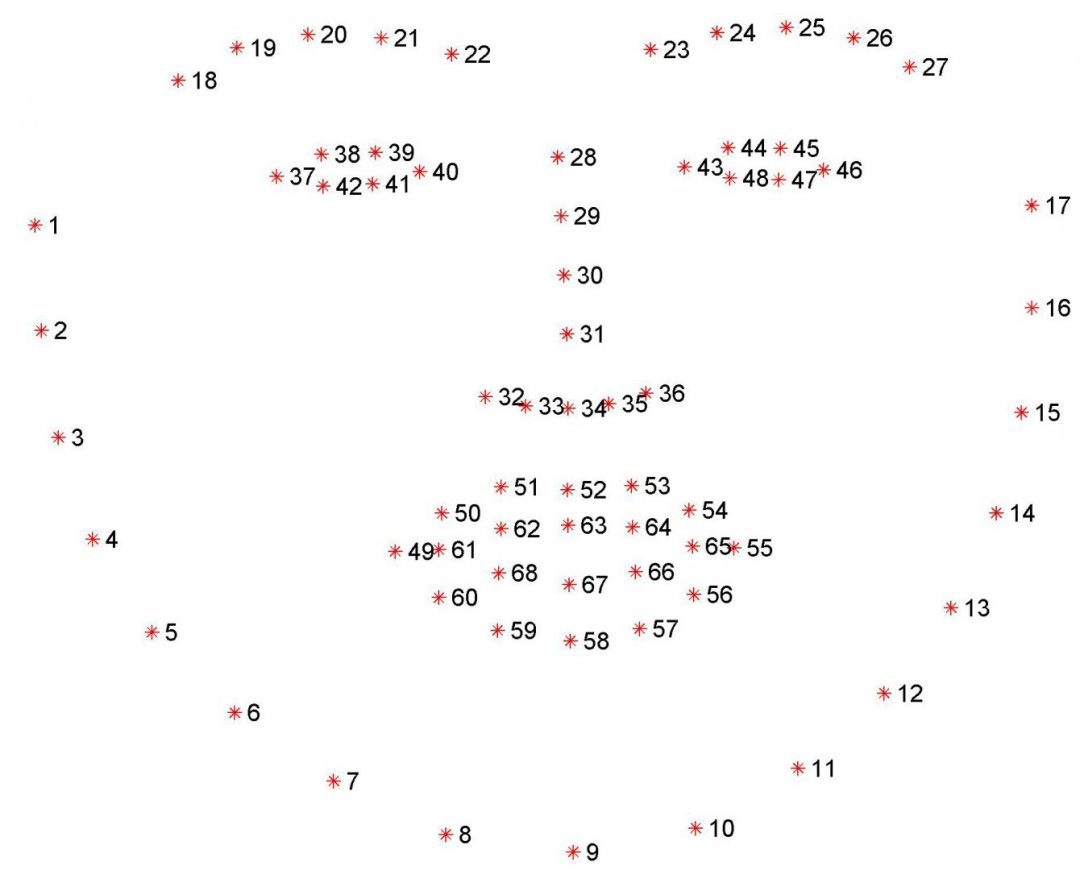
\includegraphics[scale=0.20]{chapter5/facial_landmarks.jpg}
    	\caption{An illustration showing positions of facial landmark points considered by dlib face detector. Image source: Pyimagesearch \protect\footnotemark.}
    	\label{fig_gm_pipeline}
    \end{figure}
	\footnotetext{Pyimagesearch - \url{https://pyimagesearch.com/2017/04/03/facial-landmarks-dlib-opencv-python/}}
    \subsubsection{c. Coordinate Transformation}
    The next step warps the consituent facial images in a such a way that their landmark points corresponding to the right corner of the right eye and the left corner of the left eye are shifted to locations $P_{1}$ (0.3 x image width, 0.3 x image height) and $P_{2}$ (0.7 x image width, 0.3 x image height) respectively. In practice this is achieved by computing and applying a similarity transformation matrix using OpenCV library's \enquote{estimateRigidTransform} method.
    
    Similarity transformation \cite{hartley2003multiple} is a specialization of projective transformations, composed of an euclidean transformation (rotation and translation), and an isotropic scaling. Planar similarity transformation has four Degrees Of Freedom (DOFs) can be expressed in the following form:
    <equation>
    
    Planar affine transformation has two more DOFs offered by non-isotropic scaling and shear. A planar affine transformation can represented in the form of following matrix:
    
    \subsubsection{d. Facial Alignment using Delaunay Triangulation}
    Facial images are now anchored at points $P_{1}$ and $P_{2}$. However, their regions are yet to be aligned to a common reference. Such a reference is obtained by computing the mean of landmark points of all constituent faces. Subsequently, every facial image is split into regions using Delaunay triangulation technique. \enquote{A Delaunay triangulation of a vertex set is a triangulation of the vertex set with the property that no vertex in the vertex set falls in the interior of the circumcircle (circle that passes through all three vertices) of any triangle in the triangulation}\cite{cmu_triangle:_nodate}. An affine transformation is computed for every triangular region using its vertices, to warp and fit it in the corresponding region formed by the mean landmark points.
    
    \subsubsection{e. Averaging}
    The aligned sets of images are averaged to form their corresponding composite faces.
    
    \subsection{C. Syndrome-wise Attribution Map Generation}
    Syndrome-wise attribution maps are generated using three different methods and their implementation details are discussed below.
    \subsubsection{i. Attribution Maps of Composite Faces}
    The first type of syndrome-wise maps are obtained by treating composite faces as individual patient faces and applying the patient-wise attribution map generation procedure.
    \subsubsection{ii. Average Attribution Maps}
    Average attribution map of a given syndrome is obtained by computing the mean across attribution maps of the correctly predicted instances from the class's test split.
    \subsubsection{iii. Singular Value Decomposition (SVD) of Attribution Maps}
	Eigen-CAM \cite{muhammad2020eigen} is a layer attribution technique, which computes saliency from the first principal component of feature activations of channels, across the target convolutional layer. For this experiment, we apply the same technique to the attribution maps of correct predicted samples of a given class, for obtaining its characteristic saliency map. The procedure is described in a step-wise manner below:

	\begin{enumerate}
		\item Vectorize the attribution maps of correctly predicted samples of a given syndrome class $c$ into a matrix $A_{c}$.
		\item Mean subtraction <>
		\item Factorize $A_{c}$ using SVD to compute principal components of $A_{c}$
		\begin{equation}
			A_{c} = U \Sigma {V}^T
		\end{equation}
		where $U$ is an $MXM$ orthogonal matrix and V is an $NXN$ orthogonal matrix.  The columns of $U$ and $V$ form the left and right singular vectors of $A_{c}$ respectively. The resultant attribution map $R_{c}$ is obtained by projecting $A$ on the first right eigen vector $V_{1}$:
		\begin{equation}
			R_{c} = A_{c}V_{1}
		\end{equation}
	
	The procedure is applied individually on attribution maps of all the three GradCAM, HiResCAM and FullGrad methods, for all syndromes under our scope. In the cases of average and SVD of attribution map visualizations, a given syndrome's composite face is used as the background image to project the maps, although there is no relationship between them.
	\begin{figure}[H]
		\hspace*{0cm}      
		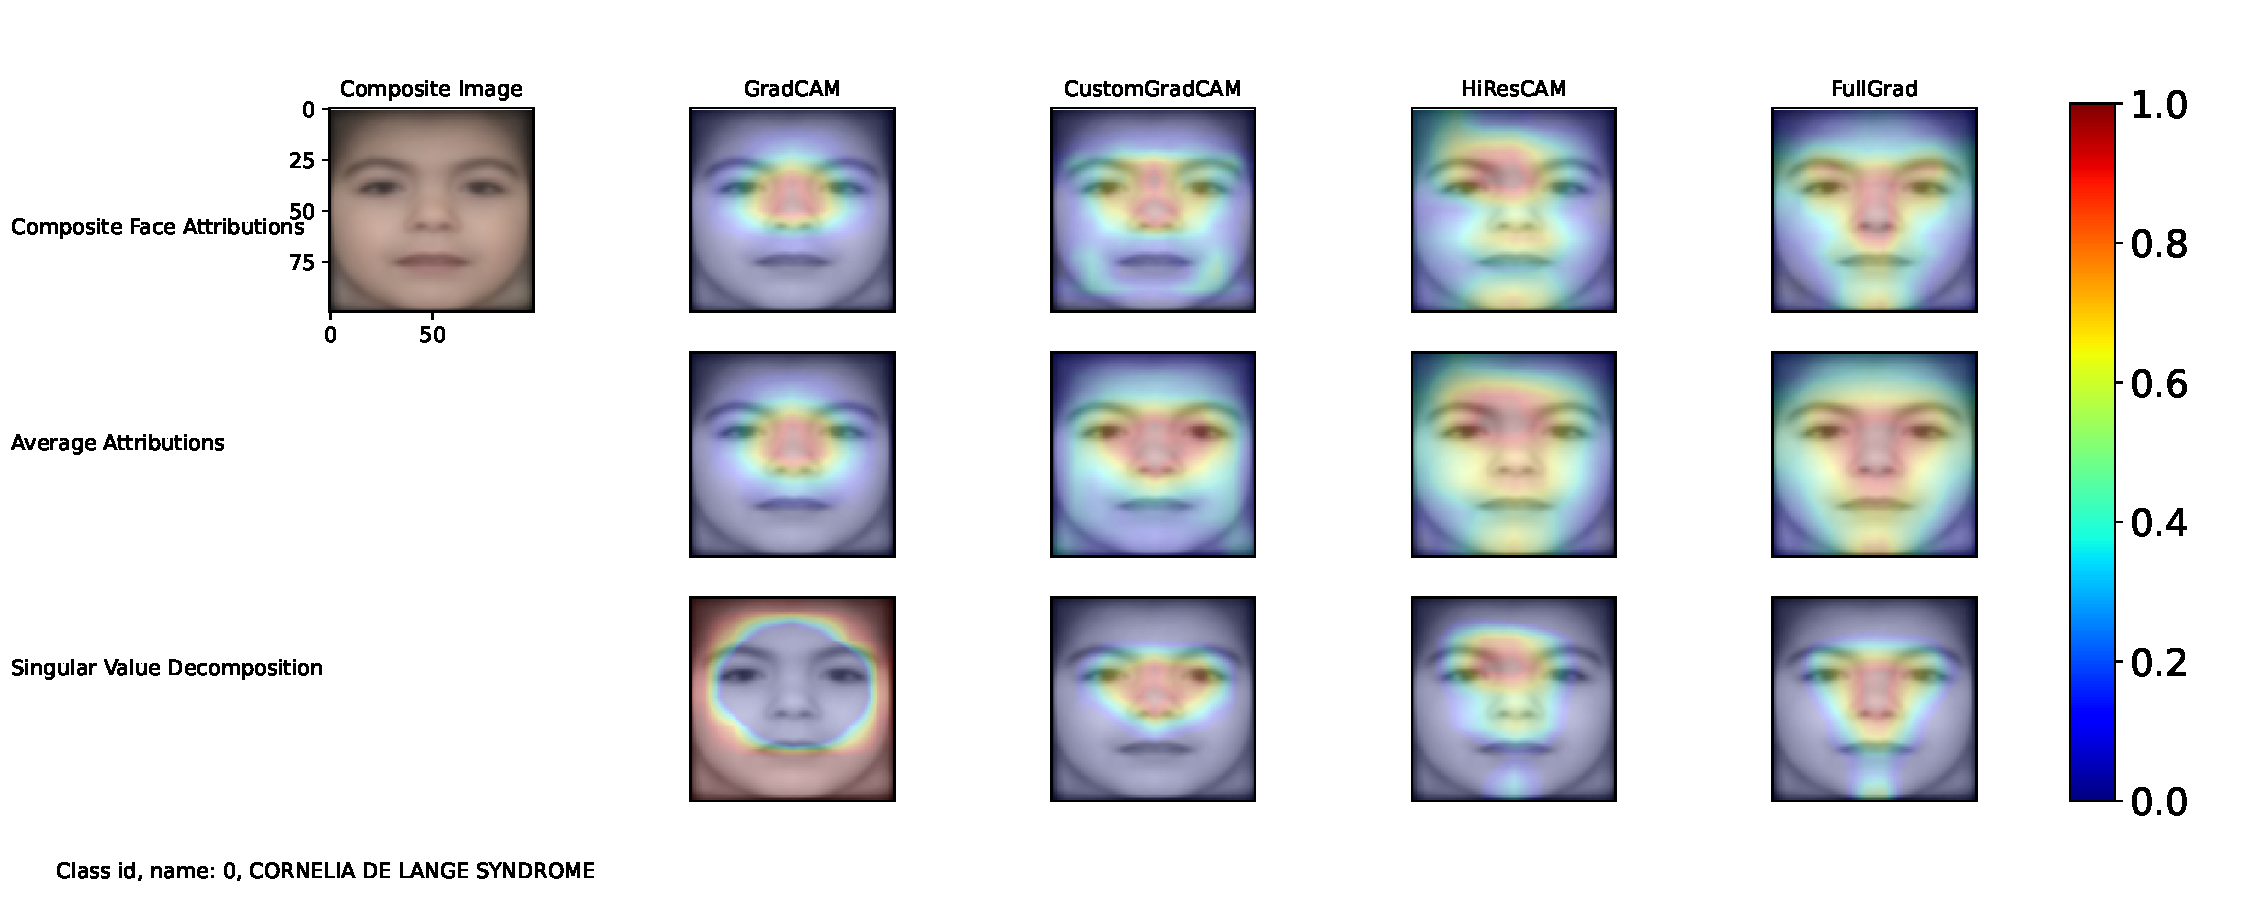
\includegraphics[scale=0.43]{chapter5/example_syndrome_wise_map.pdf}
		\caption{An example for syndrome-wise attribution maps}
		\label{fig_synd_maps}
	\end{figure}
	\end{enumerate}    
    \subsection{D. Dataset Imbalance - Explanation Quality Analysis}
    The aim of this experiment is to investigate the effects of class imbalance in GMDB on contents and quality of generated attribution maps. We trained four classifier models each with different numbers and choices for syndrome classes, using the same network architecture and hyperparameters as that of the 139 class GestaltMatcher classifier model. Table \ref{} summarizes the experimental setup.
   \section{Evaluation Questionnaire}
   We considered six genetic syndrome classes from GMDB for evaluation: Cornelia de Lange syndrome (CDLS), Williams Beuren syndrome (WBS),  Coffin-Siris syndrome (CSS),  Nicolaides-Baraitser syndrome (NBS), Hyperphosphatasia-intellectual disability syndrome or Hyperphosphatasia mental retardation syndrome (HPMRS) and Smith-Lemli-Opitz-Syndrome (SMOS). The syndromes were chosen as they make up majority classes of GMDB. Their respective composite faces, patient-wise attribution maps of correctly predicted test samples and syndrome-wise attribution maps, were compiled into a questionnaire which can be accessed at \url{https://forms.gle/aRru9aeCyZaqpURP9}. The survey was designed to be self-explanatory in nature, containing all necessary information for the evaluator.
   
   Following is an outline of the questionnaire:
   \begin{itemize}
   	\item Section 1. Professional Details and Introduction
   	\item Section 2. Composite Face Evaluation
   		\begin{itemize}
   		\item Introduction
   		\item Questions
   		\end{itemize}
   \item Section 3. Patient-wise Attribution Map Evaluation
   		\begin{itemize}
   		\item Introduction
   		\item Questions	
   		\end{itemize}
   	\item Section 4. Syndrome-wise Attribution Map Evaluation
   	\begin{itemize}
   	\item Introduction
   	\item Questions
   \end{itemize}
   \end{itemize}

   \subsubsection{Section 1. Professional Details and Introduction}
   The first section asks the evaluator (clinician) for his professional details, and gives a brief introduction to the questionnaire. Details including his professional experience, specialization and his familiarity with the syndromes presented for evaluation are collected. 
    
    
   \subsubsection{Section 2. Composite Face Evaluation}
   This section contains an introduction followed by a couple of questions. The first question asks the evaluator to identify the syndrome represented by the given composite face. Subsequently, the targeted syndrome name is revealed, and the clinician is asked whether the presented face contains its characteristic phenotypic features.
    
   \subsubsection{Section 3. Patient-wise Attribution Map Evaluation}
   This part of the questionnaire contains an introduction which briefly explains the objective of our research work to the evaluator, especially regarding the integration of XAI methods to the GestaltMatcher model. Subsequently, it presents the clinician a set of five questions for every patient-wise attribution map in the questionnaire.
   \subsubsection{Section 4. Syndrome-wise Attribution Map Evaluation}
   The final section of the questionnaire contains a background subsection followed by a question asking the evaluator to pick upto four of the twelve presented syndrome-wise maps and rank them.
   
   Tables \ref{tbl_comp_face}, \ref{tbl_pat_wise}, \ref{tbl_synd_wise} contain the list of questions included in sections 2 till 4 respectively. Each row in the tabular columns represent an individual page in the evaluation questionnaire. The first section and introductory parts of all the other three sections are provided in the appendix\ref{}.
  
    \begin{table}[H]
    	\centering
    	\begin{tabular}{ | c | m{7cm} |}
    		\hline
    		\multicolumn{2}{|c|}{\textbf{Section 2}} \\
    		\hline
    		{\centering {\textbf{Displayed Images}}} & {\centering{\textbf{Questions/Displayed Text}}} \\ \hline
		
    		\begin{minipage}{.49\textwidth}
    			\hspace{1cm}
    			\centering
    			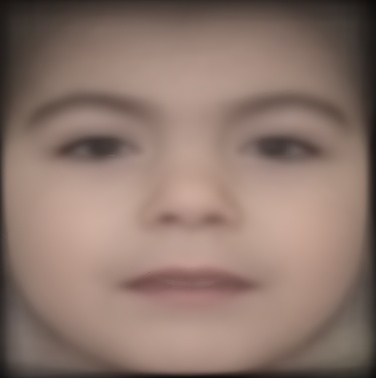
\includegraphics[scale=0.2]{chapter5/composite_face.jpg}
    			\hspace{1cm}
    		\end{minipage}
    		
    		&
    		%\begin{minipage}[t]{5cm}
    		\hspace{1cm}
    		
    		1a. What genetic syndrome do you think the given image most likely represents? (Select one)
    		\begin{itemize}
    			\item Coffin-Siris syndrome
    			\item Cornelia de Lange syndrome
    			\item Hyperphosphatasia - intellectual disability syndrome
    			\item Nicolaides Baraitser syndrome
    			\item Williams syndrome (Williams Beuren syndrome)
    			\item Smith Lemli Opitz syndrome
    			\item None
    		\end{itemize}
    		\hspace{1cm}
    		%\end{minipage}
%    		& 
%    		%\begin{minipage}{5cm}
%    		\begin{itemize}
%    			\item Accessibility
%    			\item Up to date information
%    			\item Fulfil students needs and wants \ldots
%    		\end{itemize}
    		%\end{minipage}
    		\\ \hline
    	\centering
    	\begin{minipage}{.49\textwidth}
    		\vspace*{1cm}
    		\centering
    		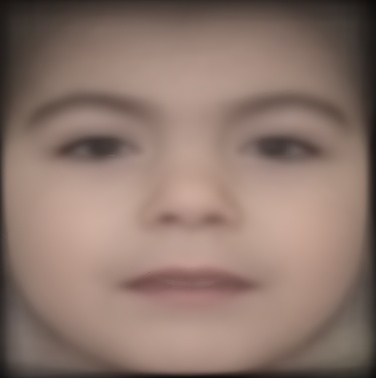
\includegraphics[scale=0.2]{chapter5/composite_face.jpg}
    		
    		\vspace*{1cm}
    	\end{minipage}
    	
    	&
    	%\begin{minipage}[t]{5cm}

    	
    	Show the true label: \enquote{The composite face represents \textbf{Cornelia de Lange syndrome}}
    	
    	
    	\\ \hline
    	\begin{minipage}{.49\textwidth}
    		\vspace*{1cm}
    		\centering
    		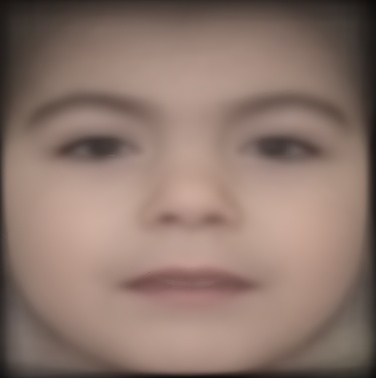
\includegraphics[scale=0.2]{chapter5/composite_face.jpg}
    		\vspace*{1cm}
    	\end{minipage}
    	
    	&
    	1b. Do you feel that the composite face contains characteristic facial features of
    	Cornelia de Lange syndrome?
    	\begin{itemize}
    		\item Yes
    		\item No
    	\end{itemize}
    	
    	\\ \hline
    	\end{tabular}
    	\caption{Questions in the composite face section of the evaluation questionnaire}\label{tbl_comp_face}
    \end{table}
    
    
    
    
    
    
    
    
    
    
%   \begin{figure}[H]
%   	\centering
%   	\begin{subfigure}[b]{0.45\textwidth}
%   		\centering
%   		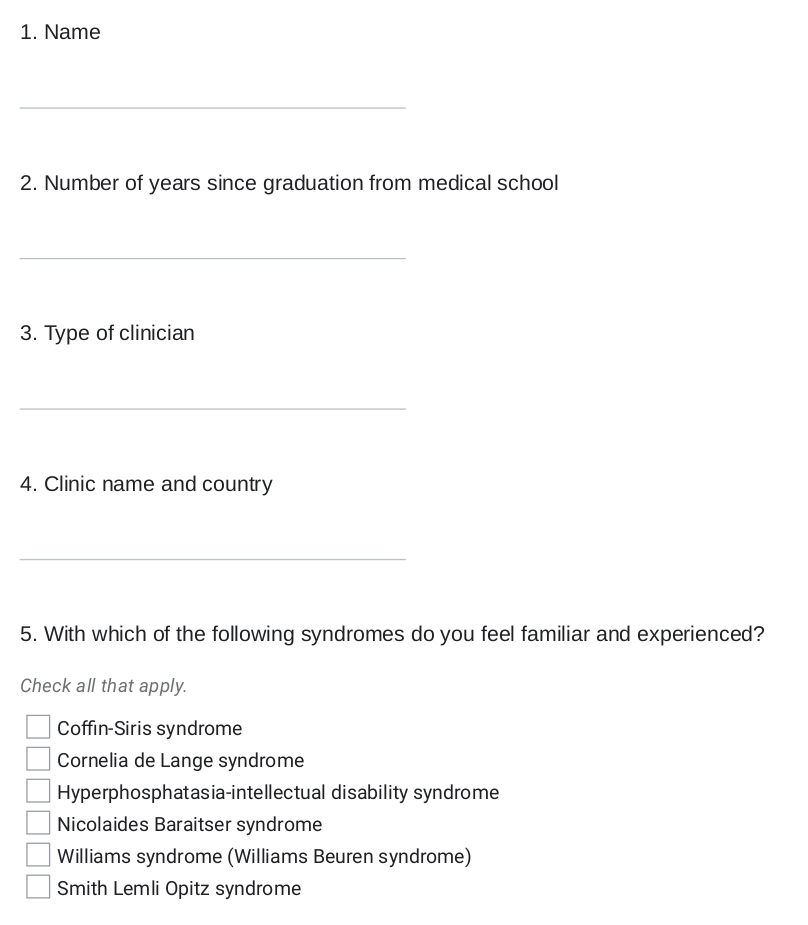
\includegraphics[width=\textwidth]{chapter5/q11.png}
%   		\caption{Professional details}
%   		\label{fig:y equals x}
%   	\end{subfigure}
%    \hfill
%   	\begin{subfigure}[b]{0.45\textwidth}
%   		\centering
%   		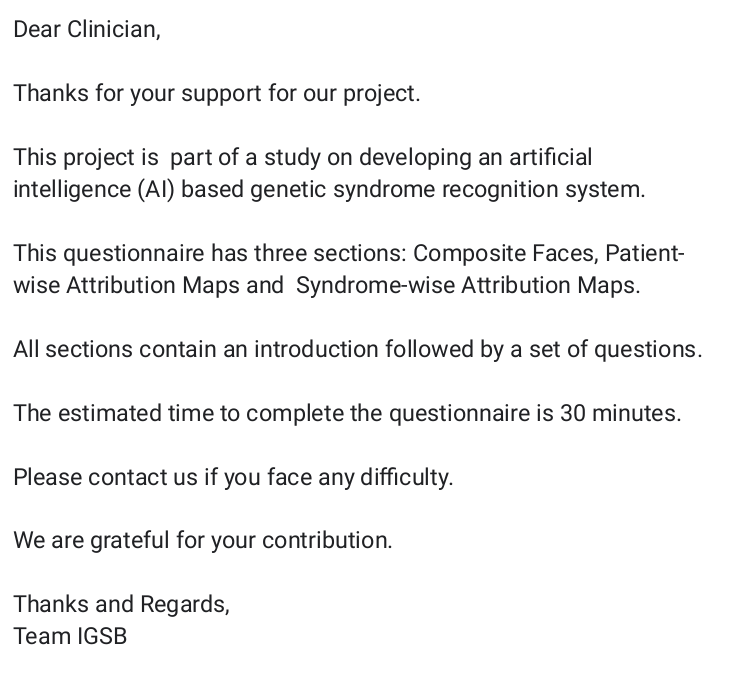
\includegraphics[width=\textwidth]{chapter5/q12.png}
%   		\caption{Questionnaire introduction}
%   		\label{fig:three sin x}
%   	\end{subfigure}
%   	\hfill
%   	\vfill
%   	\vfill
%   	\caption{Section 1 of the evaluation questionnaire}
%   \end{figure}


    \begin{table}[H]
   	\centering
   	\begin{tabular}{ | c | m{7cm} |}
   		\hline
   		\multicolumn{2}{|c|}{\textbf{Section 3}} \\
   		\hline
   		{\centering {\textbf{Displayed Images}}} & {\centering{\textbf{Questions/Displayed Text}}} \\ \hline
   		
   		\begin{minipage}{.49\textwidth}
   			\hspace{1cm}
   			\centering
   			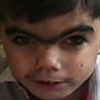
\includegraphics[scale=0.9]{chapter5/patient_1.jpg}
   			\hspace{1cm}
   		\end{minipage}
   		
   		&
   		%\begin{minipage}[t]{5cm}
   		\hspace{1cm}
   		
   		2a. What genetic syndrome do you think the given most likely represents? (Select one)
   		\begin{itemize}
   			\item Coffin-Siris syndrome
   			\item Cornelia de Lange syndrome
   			\item Hyperphosphatasia - intellectual disability syndrome
   			\item Nicolaides Baraitser syndrome
   			\item Williams syndrome (Williams Beuren syndrome)
   			\item Smith Lemli Opitz syndrome
   			\item None
   		\end{itemize}
   		\vspace{.5cm}
   		2b. What phenotypic features were considered most important for your choice?
   		\vspace{.5cm}
   		%\end{minipage}
   		%    		& 
   		%    		%\begin{minipage}{5cm}
   		%    		\begin{itemize}
   			%    			\item Accessibility
   			%    			\item Up to date information
   			%    			\item Fulfil students needs and wants \ldots
   			%    		\end{itemize}
   		%\end{minipage}
   		\\ \hline
   		
   		\centering
   		\begin{minipage}{.49\textwidth}
   			\vspace*{1cm}
   			\centering
   			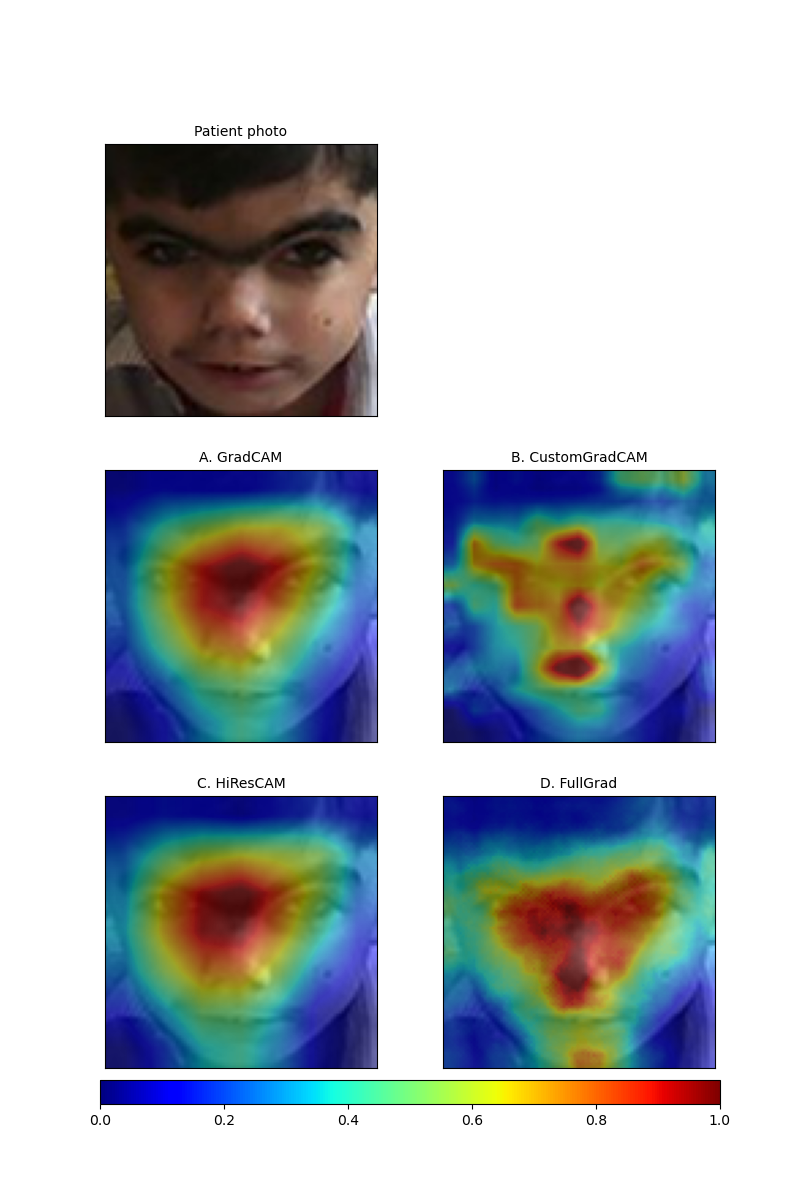
\includegraphics[scale=0.3, trim = 0cm 3cm 0cm 3cm, clip]{chapter5/patient_map.png}
   			
   			\vspace*{1cm}
   		\end{minipage}
   		
   		&
   		%\begin{minipage}[t]{5cm}
   		
   	   		
   		2c. Do you change your diagnosis after seeing the attribution maps?
   		\begin{itemize}
   			\item Yes
   			\item No
   		\end{itemize}
   		\\ \hline
   	\end{tabular}
   \end{table}
   	\pagebreak
   	
   	\begin{table}
   	
   \begin{tabular}{ | c | m{7cm} |}
   		\hline
	\begin{minipage}{.49\textwidth}
	\vspace*{1cm}
	\centering
	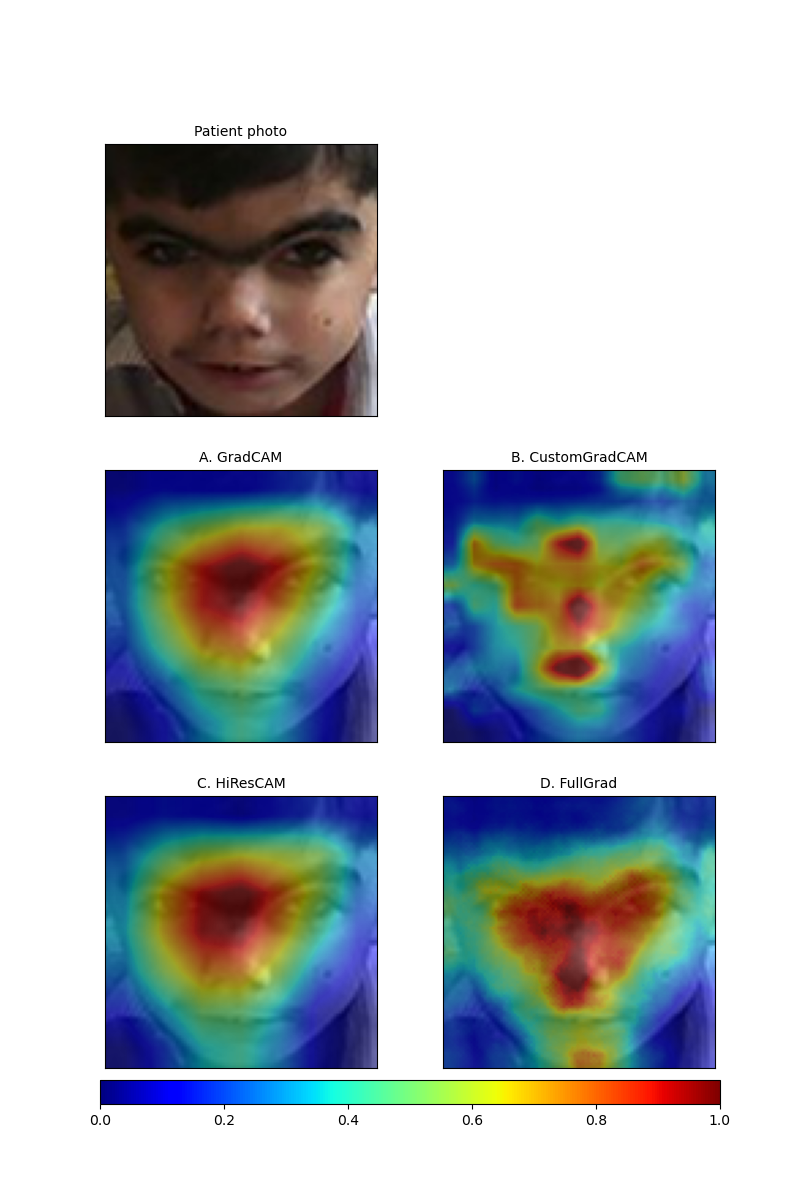
\includegraphics[scale=0.3, trim = 0cm 3cm 0cm 3cm, clip]{chapter5/patient_map.png}
	
	\vspace*{0.5cm}
\end{minipage}
   	
   	&
   	\vspace{.25cm}
   	Show the true label: \enquote{The patient has \textbf{Cornelia de Lange syndrome}}
   	
   	\vspace{.25cm}
   	
   	2d. Which of the attribution maps shown best highlights the important phenotypic
   	features (those used for diagnosis) of the above mentioned syndrome in the patient ?
   	(Rank them from 1 to 4 (with 1 as the top choice)). If you feel that none of them
   	highlight the key features select None in all rows)
   	
   	<Options A till D to assigned ranks>
   			
   	\vspace{.2cm}
   	2e. Do you find attribution maps to be helpful in evaluating the image?
   	\vspace{.5cm}
   	\\ \hline
   \end{tabular}
   	\caption{Questions in the patient-wise maps section of the evaluation questionnaire}\label{tbl_pat_wise}
   \end{table}
   
%    \begin{figure}[H]
%    \hspace*{0.5cm}  
%   	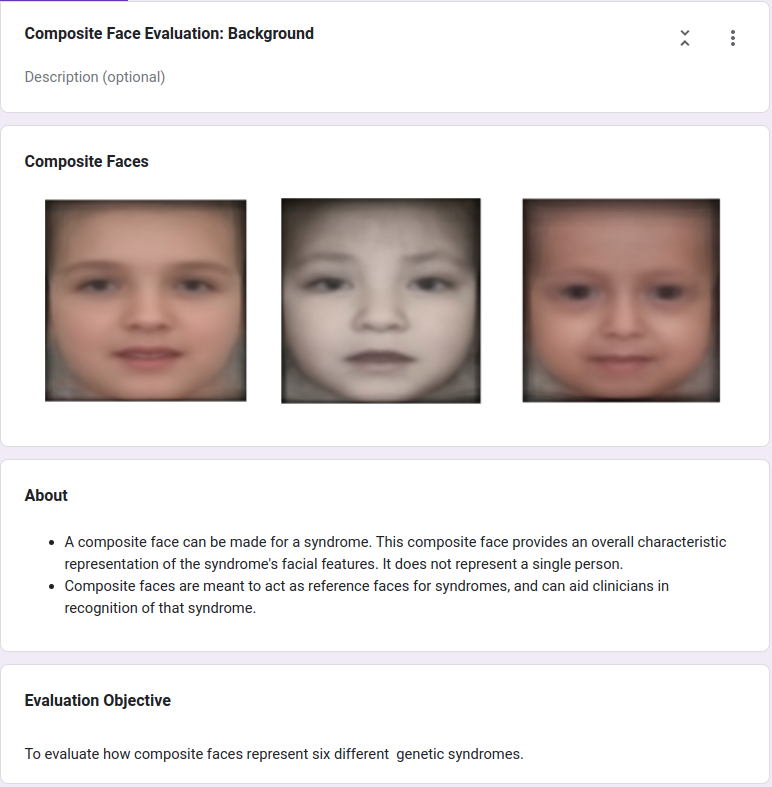
\includegraphics[scale=0.55]{chapter5/q21.png}
%   	\caption{Introductory part of the composite face section of the evaluation questionnaire}
%   	\label{fig_gm_pipeline}
%   \end{figure}
%      \begin{figure}[H]
%   	\begin{subfigure}[b]{0.47\textwidth}
%   		\centering
%   		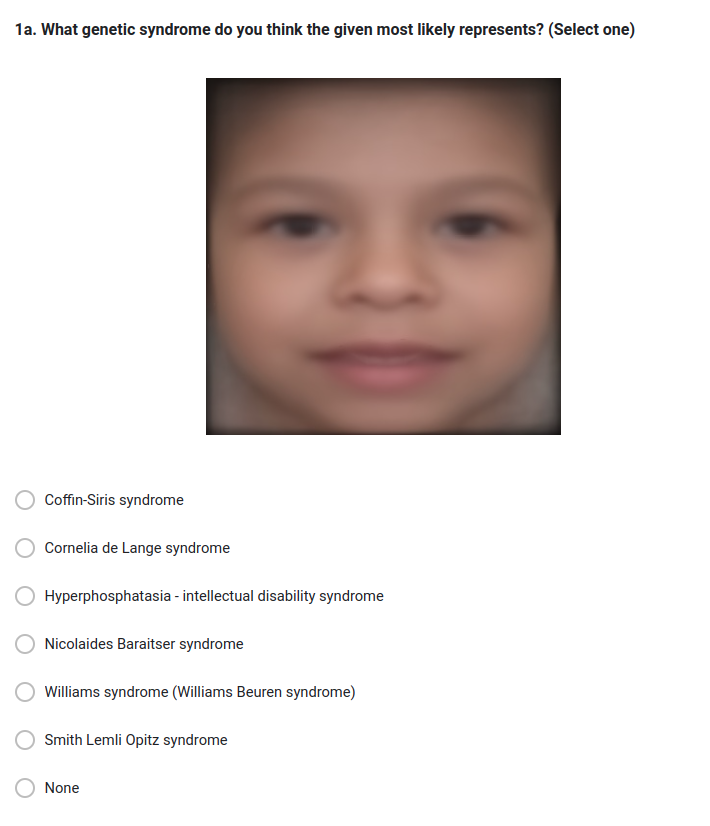
\includegraphics[width=\textwidth,trim = 0cm 0cm 2cm 0cm, clip]{chapter5/q22.png}
%   		\caption{Professional details}
%   		\label{fig:y equals x}
%   	\end{subfigure}
%	\hfill
%   	\begin{subfigure}[b]{0.47\textwidth}
%   		\centering
%   		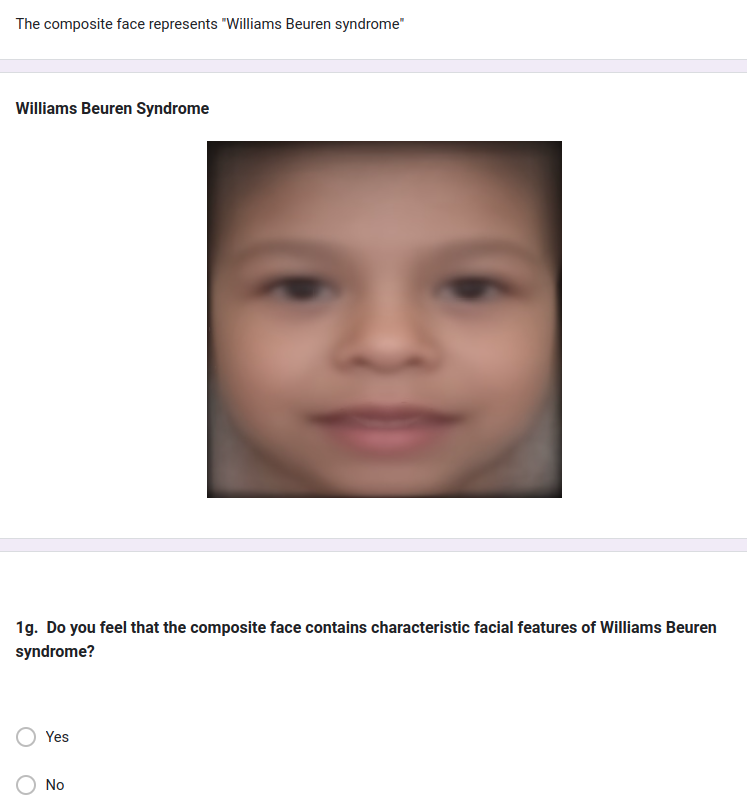
\includegraphics[width=1.1\textwidth,trim = 0cm 0cm 1cm 0cm, clip]{chapter5/q23.png}
%   		\caption{Questionnaire introduction}
%   		\label{fig:three sin x}
%   	\end{subfigure}
%   	\caption{Section 1 of the evaluation questionnaire}
%   \end{figure}
       \begin{table}[H]
   	\centering
   	\begin{tabular}{ | c | m{7cm} |}
   		\hline
   		\multicolumn{2}{|c|}{\textbf{Section 4}} \\
   		\hline
   		{\centering {\textbf{Displayed Images}}} & {\centering{\textbf{Questions/Displayed Text}}} \\ \hline
		\begin{minipage}{.49\textwidth}
			\vspace*{1cm}
			\centering
			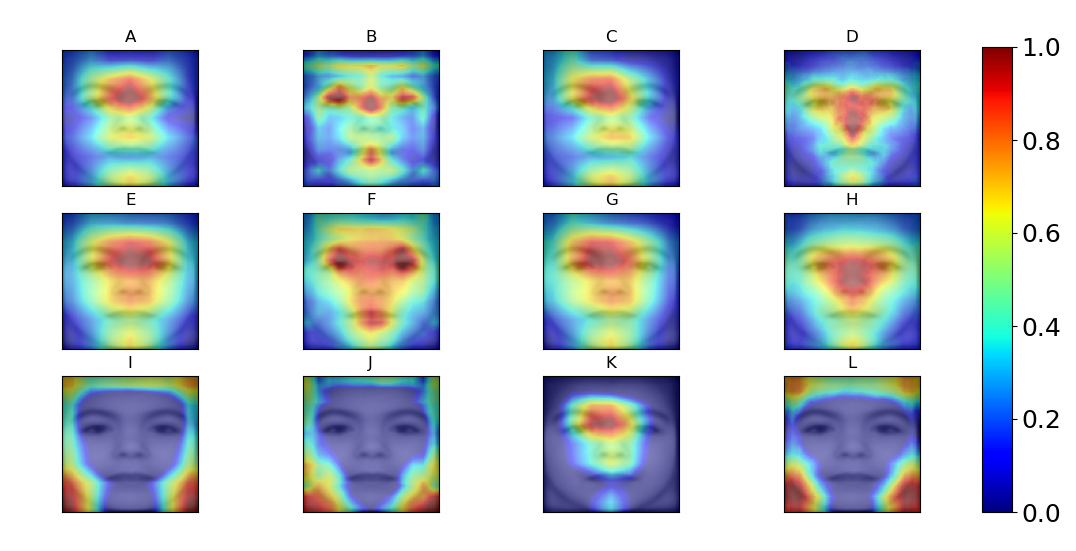
\includegraphics[scale=0.3, trim = 1cm 0cm 0cm 0cm, clip]{chapter5/syndrome_map.png}
			\vspace*{0.5cm}
		\end{minipage}
		
		&

		
		3. Which of the  attribution maps shown below most highlight the key characteristic facial phenotypic features of Cornelia de Lange syndrome? (Select top four. If none of them represent select None in all rows))
		
		<Top four from A till L to be selected>		
		
		\vspace{.25cm}
		\\ \hline
	\end{tabular}
	\caption{Questions in the syndrome-wise maps section of the evaluation questionnaire}\label{tbl_synd_wise}
\end{table}
\end{document}
